%!TEX root = main.tex

\section{Revisão da Literatura}

A revisão de literatura consiste na apresentação, síntese e avaliação crítica da dita literatura, de modo a sustentar, de um ponto de vista teórico, a investigação efetuada.

É importante de referir que a cultura organizacional de uma empresa influência a própria organização. Deste modo, a cultura pode ser definida como um conjunto de ideias adquiridas ao longo do tempo que distinguem membros de diferentes grupos e a sua forma de reagir a diferentes situações \parencite{Schein_1990,Ravasi_Schultz_2006}.

As cultura organizacionais podem ser classificadas, subdivididas e comparadas através de vários modelos e teorias avançadas pela comunidade académica. Neste relatório e, no processo de análise da empresa em questão, vamos enquadrar a mesma em três modelos: o modelo de Cameron \& Quinn, o modelo Ogbonna \& Harris e o modelo de Hofstede.

\subsection{Modelo de Cameron \& Quinn}

O modelo de Cameron \& Quinn \parencite{Cameron_Quinn_2011} define quatro tipos de culturas organizacionais, baseados na \acrfull{cvf} (inicialmente desenvolvido por professores na Universidade de Michigan \parencite{10.2307/3380029}). Estes quatro tipos de culturas podem ser representados num sistema de duas dimensões.

\begin{figure}[h]
\centering
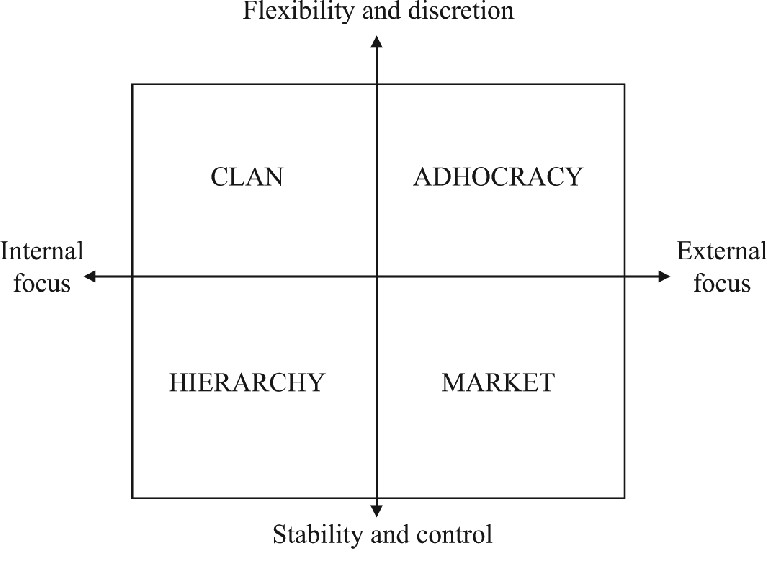
\includegraphics[width=0.5\textwidth]{cvf}
\caption{Modelo de Cameron \& Quinn}
\end{figure}

Estas dimensões definem uma dicotomia entre duas características de uma organização. Assim, a dimensão da flexibilidade/estabilidade impõe uma divisão entre organizações mais flexíveis e adaptáveis e, em contrapartida, organizações mais estáveis e controladoras. A dimensão de foco define uma dicotomia entre um foco de uma organização em processos internos ou em processos externos \parencite{diagnosing}.

Com estas divisões feitas, podemos definir os 4 tipos de culturas organizacionais:

\begin{itemize}
	\item \textit{Clan}
	\item \textit{Adhocracy}
	\item \textit{Hierarchy}
	\item \textit{Market}
\end{itemize}

\subsubsection{\textit{Clan}}

Esta cultura é definida por ter um foco interno e flexibilidade na manutenção da organização. Direciona-se para as pessoas afetas à organização. Esta tipologia é identificada, de forma geral, em organizações familiares.


\subsubsection{\textit{Adhocracy}}

Esta tipologia define uma cultura flexível e focada no mercado. Dá especial importância à inovação e empreendedorismo. Este tipo de organização é encontrado em mercados em rápido crescimento e com uma baixa aversão a risco.

\subsubsection{\textit{Hierarchy}}

Esta tipologia define uma cultura estável, controlada e com um foco interno. Enfatiza a eficiência e controlo dos processos organizacionais e a eliminação de erros. Este tipo de organização representa em grande parte organizações burocráticas com estruturas rígidas e bem-definidas.

\subsubsection{\textit{Market}}

Esta tipologia define uma cultura estável, controlado e com um foco no mercado. Assim, a organização está direcionada para a competição, em atingir objetivos. Esta tipologia adequa-se a empresas de marketing e vendas, por exemplo.

\subsection{Modelo de Ogbonna \& Harris}

\subsection{Modelo de Hofstede}


